\chapter{Linear Functions and Slope}

\section{Equations of Lines}

Write the equation of each line \textbf{in point-slope form} that goes through each pair of points.
\begin{enumerate}
\item $(-2, 1), \, (7,8)$
\item $(0,4), \, (9,-15)$
\item $(-1,-2), \, (-3,-13)$
\end{enumerate}

\section{Average Rate of Change}

Recall that when you evaluate a function at a point, such as evaluating $f(x) = -3x^2 - 2x + 4$ when $x = 1$, you get
\begin{align*}
    f(x) &= -3x^2 - 2x + 4 \\
    f(1) &= -3(1)^2 - 2(1) + 4 \\
    &= -1
\end{align*}

If we look at the graph of the function, the point $(1, -1)$ is on the graph.

\begin{center}
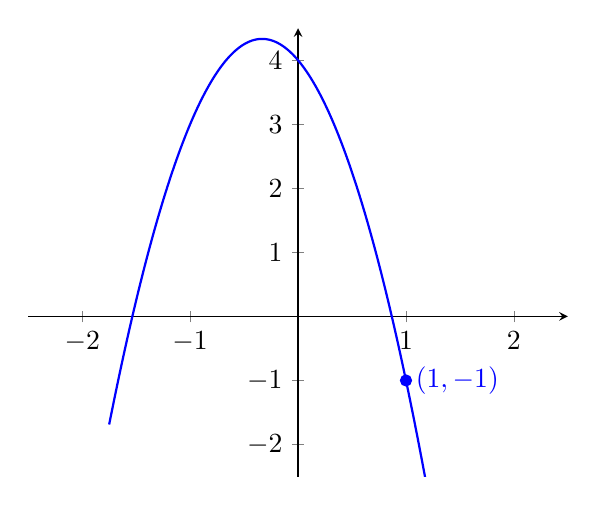
\begin{tikzpicture}
\begin{axis}
[axis lines = middle, xmin = -2.5, xmax = 2.5, ymin = -2.5, ymax = 4.5, xtick distance = 1, ytick distance = 1]
\addplot[thick, blue, domain=-1.75:1.25, samples=200] plot {-3*x^2 - 2*x + 4};
\addplot[mark=*, blue] coordinates {(1,-1)} node [right] {$(1,-1)$};
\end{axis}
\end{tikzpicture}
\end{center}

The average rate of change of a function $f(x)$ is the \textbf{slope} of the line connecting two points on the graph:
\bigskip 

\[
\text{Average rate of change = slope = } \frac{f(x_2)-f(x_1)}{x_2-x_1}
\]

\newpage 

\begin{example}
Find the average rate of change of $f(x) = -3x^2-2x+4$ in each interval.
\begin{multicols}{2}
\begin{enumerate}[(a)]
    \item $[0,1]$
    \item $[-2,1]$
\end{enumerate}
\end{multicols}
\end{example}

\begin{solution}

(a) Given $f(x) = -3x^2-2x+4$, we want to find the slope of the red line connecting the points $(0, f(0))$ and $(1, f(1))$.

\begin{center}
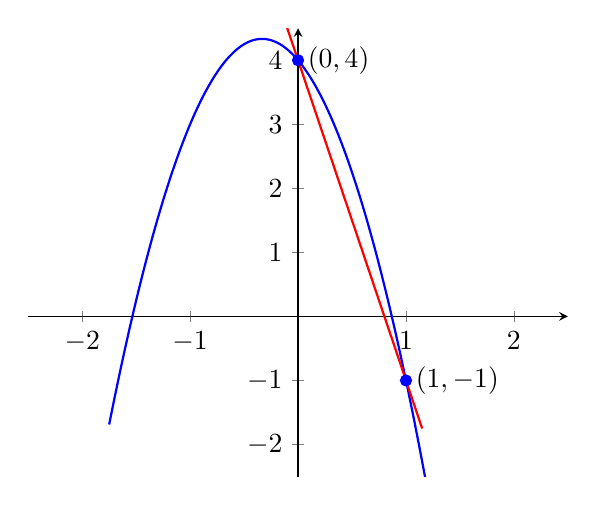
\begin{tikzpicture}
\begin{axis}
[axis lines = middle, xmin = -2.5, xmax = 2.5, ymin = -2.5, ymax = 4.5, xtick distance = 1, ytick distance = 1]
\addplot[thick, blue, domain=-1.75:1.25, samples=200] plot {-3*x^2 - 2*x + 4};
\addplot[mark=*, only marks, blue] coordinates {(1,-1) (0,4)};
\node at (axis cs:0,4) [right] {$(0,4)$};
\node at (axis cs:1,-1) [right] {$(1,-1)$};
\addplot[thick, red, domain=-0.25:1.15] plot {-5*x+4};
\end{axis}
\end{tikzpicture}
\end{center}

Noting that $f(0) = 4$, we have

\begin{align*}
    \frac{f(x_2)-f(x_1)}{x_2-x_1} &= \frac{4-(-1)}{1-0} \\[4pt]
    &= -5
\end{align*}

Thus, the average rate of change of $f(x) = -3x^2-2x+4$ over the interval $[0,1]$ is $\boxed{-5}$ \newline 

(b) This time, we want to find the slope of the red line connecting the points $(-2, f(-2))$ and $(1, f(1))$.

\begin{center}
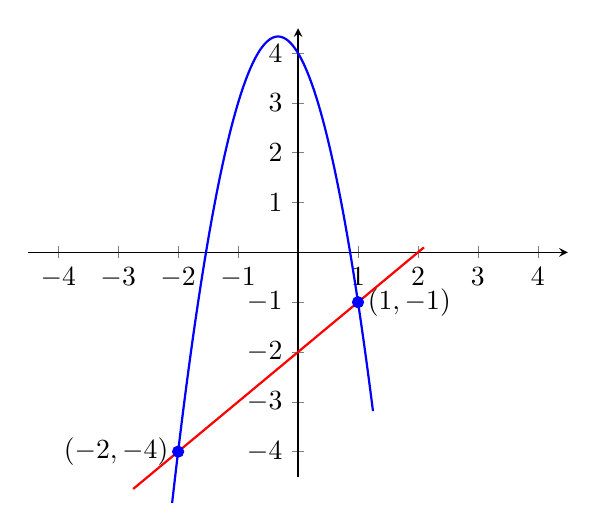
\begin{tikzpicture}
\begin{axis}
[axis lines = middle, xmin = -4.5, xmax = 4.5, ymin = -4.5, ymax = 4.5, xtick distance = 1, ytick distance = 1, clip=false]
\addplot[thick, blue, domain=-2.1:1.25, samples=200] plot {-3*x^2 - 2*x + 4};
\addplot[mark=*, only marks, blue] coordinates {(1,-1) (-2,-4)};
\node at (axis cs:-2,-4) [left] {$(-2,-4)$};
\node at (axis cs:1,-1) [right] {$(1,-1)$};
\addplot[thick, red, domain=-2.75:2.1] plot {x-2};
\end{axis}
\end{tikzpicture}
\end{center}

Noting that $f(-2) = -4$, we have

\begin{align*}
    \frac{f(x_2)-f(x_1)}{x_2-x_1} &= \frac{-1-(-4)}{1-(-2)} \\[4pt]
    &= 1
\end{align*}

Thus, the average rate of change of $f(x) = -3x^2-2x+4$ over the interval $[-2,1]$ is $\boxed{1}$

\end{solution}

\section{Exercises}

For the function $f(x) = x^2$, compute the average rate of change for each interval.
\begin{enumerate}
\item $[1, 1.1]$
\item $[1, 1.01]$
\item $[1, 1.001]$
\item $[1,1.0001]$
\setcounter{Review}{\value{enumi}}
\end{enumerate}

\begin{enumerate}
\setcounter{enumi}{\value{Review}}
\item For your answers in the previous four problems, what value do your average rates of change get closer and closer to?
\setcounter{Review}{\value{enumi}}
\end{enumerate}

Find the average rate of change of the function $f(x) = -6x^2 + 7x + 4$ over each specified interval.
\begin{enumerate}
\setcounter{enumi}{\value{Review}}
\item $[-2, -1]$
\item $[5, 6]$
\item $[0, 1]$
\item $[5,5.001]$
\item $[5,5.0001]$
\item $[5,5.00001]$
\item What value are your last 3 answers getting closer to?
\setcounter{Review}{\value{enumi}}
\end{enumerate}

For the function $f(x) = -3x^2 + 5$, determine the average rate of change of each over the given interval.
\begin{enumerate}
\setcounter{enumi}{\value{Review}}
    \item $[7, 7.001]$
    \item $[7, 7.0001]$
    \item $[7, 7.00001]$
\setcounter{Review}{\value{enumi}}
\end{enumerate}

\begin{enumerate}
\setcounter{enumi}{\value{Review}}
\item For your answers in the previous three problems, what value do your average rates of change get closer and closer to?
\setcounter{Review}{\value{enumi}}
\end{enumerate}

Given $f(x) = \sqrt{x}$, find the average rate of change of each over the given interval.
\begin{enumerate}
\setcounter{enumi}{\value{Review}}
	\item $[1, 1.0001]$
	\item $[1, 1.00001]$
	\item $[1, 1.000001]$
\setcounter{Review}{\value{enumi}}
\end{enumerate}

\begin{enumerate}
\setcounter{enumi}{\value{Review}}
\item For your answers in the previous three problems, what value do your average rates of change get closer and closer to?
\setcounter{Review}{\value{enumi}}
\end{enumerate}


Given $f(x) = 6\sqrt{x}$, find the average rate of change of each over the given interval.
\begin{enumerate}
\setcounter{enumi}{\value{Review}}
	\item $[25,\, 25.1]$
	\item $[25, \, 25.01]$
	\item $[25, \, 25.001]$
\setcounter{Review}{\value{enumi}}
\end{enumerate}

\begin{enumerate}
\setcounter{enumi}{\value{Review}}
\item For your answers in the previous three problems, what value do your average rates of change get closer and closer to?
\setcounter{Review}{\value{enumi}}
\end{enumerate}

Find the average rate of change of the function $f(x) = -7x^3 + 6\sqrt{3x} + 4$ over each interval. Round your answers to 4 decimal places.
\begin{enumerate}	\setcounter{enumi}{\value{Review}}
	\item $[0,1]$
	\item $[10,11]$
	\item $[8,15]$
\end{enumerate}	\setcounter{Review}{\value{enumi}}

\newpage

\section{Answer Key}

\subsection*{Equations of Lines}
\begin{enumerate}
\item $y-1 = \frac{7}{9}(x+2)$ \text{ or } $y-8=\frac{7}{9}(x-7)$
    \item $y-4 = -\frac{19}{9}(x-0)$ \text{ or } $y+15=-\frac{19}{9}(x-9)$
    \item $y+2 = \frac{11}{2}(x+1)$ \text{ or } $y+13=\frac{11}{2}(x+3)$
\end{enumerate}

\subsection*{Average Rate of Change}
\begin{multicols}{3}
\begin{enumerate}
\item 2.1
\item 2.01
\item 2.001
\end{enumerate}	\setcounter{Review}{\value{enumi}}
\end{multicols}
\begin{multicols}{3}
\begin{enumerate}	\setcounter{enumi}{\value{Review}} 
\item 2.0001
\item 2
\item 25
\end{enumerate}	\setcounter{Review}{\value{enumi}}
\end{multicols}
\begin{multicols}{3}
\begin{enumerate}	\setcounter{enumi}{\value{Review}} 
\item $-59$
\item 1
\item $-53.006$
\end{enumerate}	\setcounter{Review}{\value{enumi}}
\end{multicols}
\begin{multicols}{3}
\begin{enumerate}	\setcounter{enumi}{\value{Review}} 
\item $-53.0006$
\item $-53.00006$
\item $-53$
\end{enumerate}	\setcounter{Review}{\value{enumi}}
\end{multicols}
\begin{multicols}{3}
\begin{enumerate}	\setcounter{enumi}{\value{Review}} 
\item $-42.003$
\item $-42.0003$
\item $-42.00003$
\end{enumerate}	\setcounter{Review}{\value{enumi}}
\end{multicols}
\begin{multicols}{3}
\begin{enumerate}	\setcounter{enumi}{\value{Review}} 
\item $-42$
\item $-0.499988$
\item $-0.4999988$
\end{enumerate}	\setcounter{Review}{\value{enumi}}
\end{multicols}
\begin{multicols}{3}
\begin{enumerate}	\setcounter{enumi}{\value{Review}} 
\item $-0.49999988$
\item $-0.5$
\item $0.5994$
\end{enumerate}	\setcounter{Review}{\value{enumi}}
\end{multicols}
\begin{multicols}{3}
\begin{enumerate}	\setcounter{enumi}{\value{Review}} 
\item $0.59999$
\item $0.6$
\item $0.6$
\end{enumerate}	\setcounter{Review}{\value{enumi}}
\end{multicols}
\begin{multicols}{3}
\begin{enumerate}	\setcounter{enumi}{\value{Review}} 
\item 3.3923
\item $-2,315.3960$
\item $-2861.4492$
\end{enumerate}
\end{multicols}